
\section{Similarity Concentrator}
\label{sec:sic}


After semantic-level token pruning, subsequent FC layers operate seamlessly on the reduced token set, as the pruning is token-aligned and preserves structural layout. However, semantic pruning alone does not address fine-grained redundancy at the vector level. In contrast, \textbf{Similarity Concentration} targets vector-wise redundancy by matching and merging similar output vectors within local regions across frames.

Different from semantic pruning, where unimportant tokens are discarded, similar vectors often carry essential information and thus require accurate removal and later reconstruction. To support this, the similarity process includes two core components:
\textbf{Similarity Gather}: removes similar vectors and constructs a compact output.
\textbf{Similarity Scatter}: restores the original full layout using a similarity map.


\subsection{{Similarity Gather}}
\label{subsec:gather}
In this section, we first detail the design of \textbf{Similarity Gather}, which efficiently operates in a fully streaming fashion.

\textbf{GEMM Tiling.}  
As shown in \Fig{fig:sic_gather}(1), Similarity Gather operates on the output of GEMM\footnote{{Similarity Gather on output of FFN, O projection, and PV GEMM}}. Assume the input has dimension $M \times K$, the weight matrix is $K \times N$, and the output is $M \times N$. 
Due to limited on-chip resources, we adopt a tiling strategy widely used in modern accelerators~\cite{chen2016eyeriss,jouppi2017datacenter}. 
Specifically, the input and weight tiles are of size $m \times K$ and $K \times n$, and the output tile is $m \times n$, where we typically set $m = 1024$ and $n = 32$.
The PE array performs one output tile at a time, producing $a$-length output vectors, where $a = n = 32$ in our implementation. {These vectors are then streamed to the Similarity Gather logic for processing when an output tile gets ready}.


\begin{figure*}[t]
    \centering
    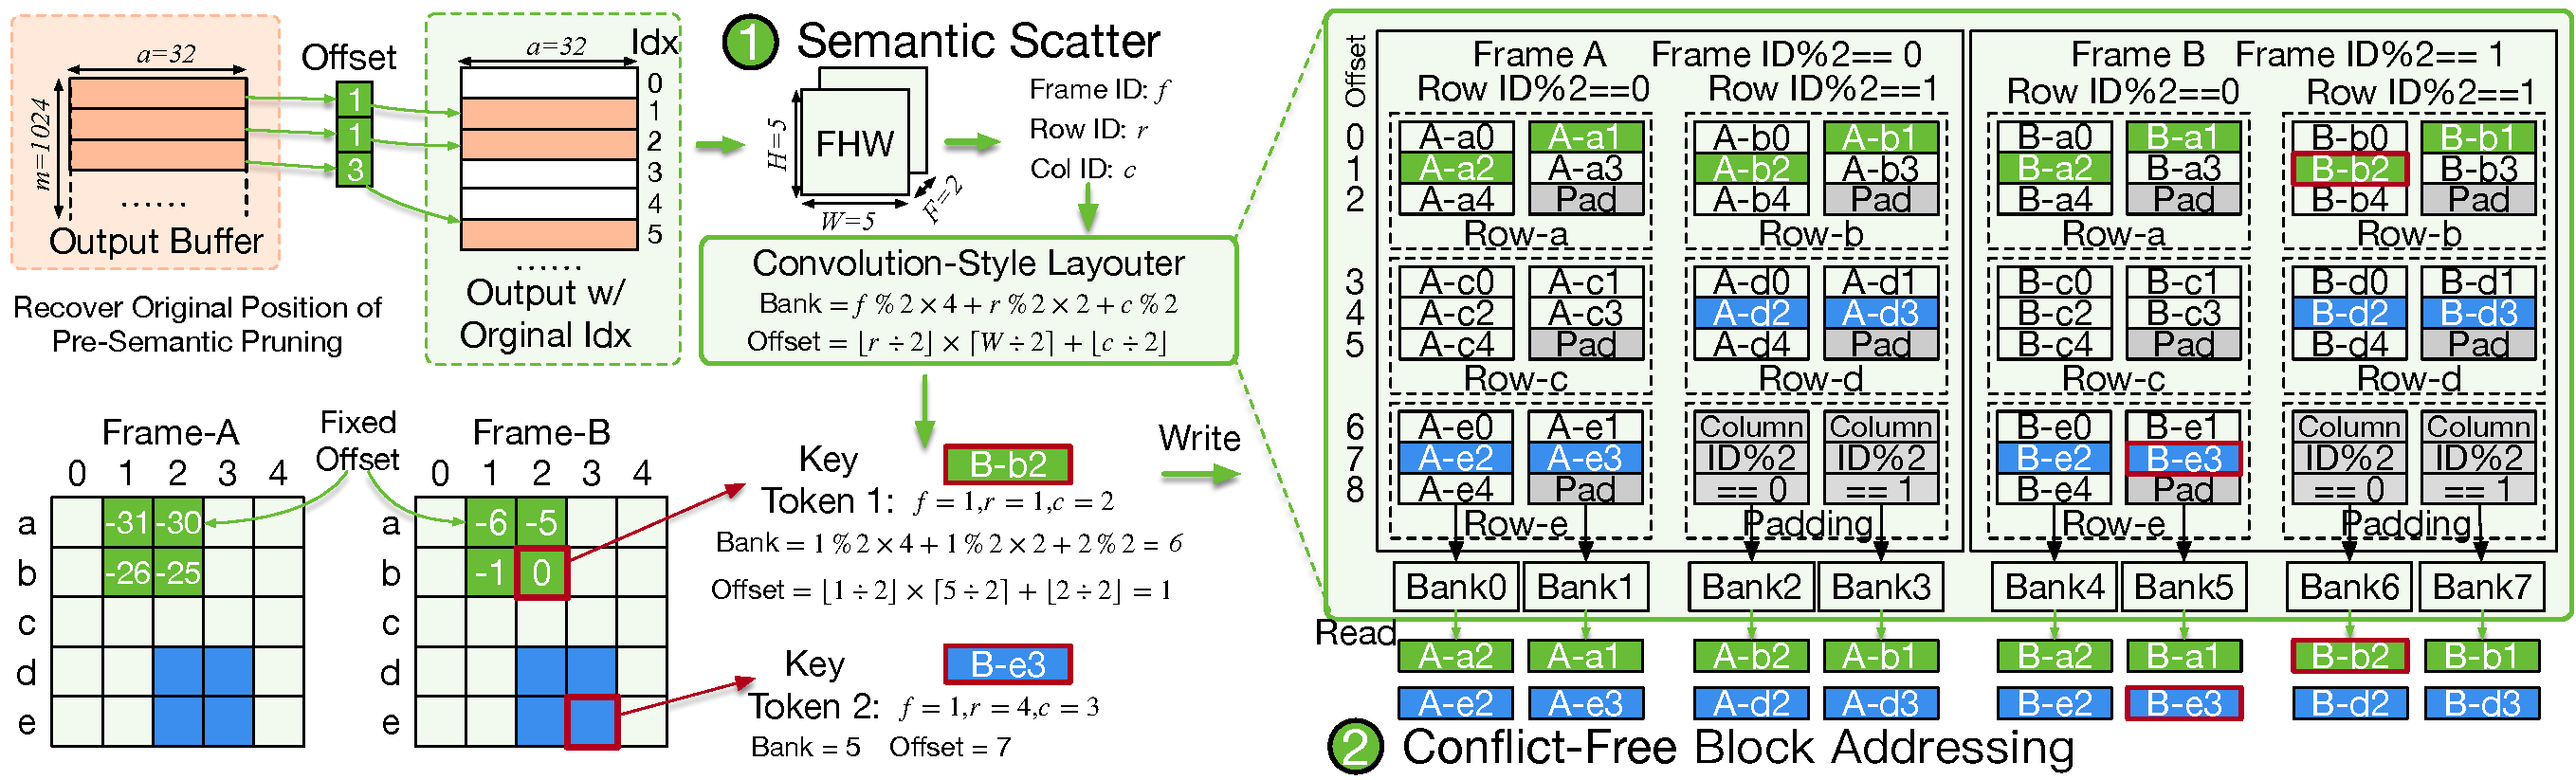
\includegraphics[width=\linewidth]{figure/sic_layouter.pdf}
    % \vspace{-7mm}
    \caption{The convolution-style layouter enables accurate token positioning and conflict-free memory access for block-level similarity. (1) Reconstructs token positions via semantic offsets and maps outputs to a FHW-layout. (2) Enables conflict-free addressing across memory banks without data duplication.}
    \label{fig:sic_layouter}
    % \vspace{-5mm}
\end{figure*}


\textbf{Block-wise Addressing.}  
To exploit spatiotemporal redundancy, we adopt a \textbf{convolution-style layout} over two adjacent frames, as illustrated in \Fig{fig:sic_gather}(2). 
{A $2 \times 2 \times 2$ sliding window spans both spatial and temporal dimensions with a stride of 1, forming a block that contains 8 vectors, 4 from each frame. 
Each element in the block is an $a$-dimensional output vector produced by the GEMM operation, and the block serves as a localized comparison group for redundancy detection.}

To efficiently support this structure, GEMM outputs are dynamically reorganized into the convolution-style layout using a dedicated reordering module, as detailed in \Sec{subsec:layout}. 
Within each block, the vector with the highest index (e.g., token ID 32) is selected as the key vector and compared against the other 7 vectors in the same block (e.g., token IDs 1 through 31) to identify potential redundancy.

\textbf{Vector-wise Similarity Matching.}  
As shown in \Fig{fig:sic_gather}(3), each key vector is streamed into the \textbf{Similarity Matcher}, which performs localized comparisons to determine whether the vector is redundant. 
We adopt cosine similarity to compare two vectors $\mathbf{p}$ and $\mathbf{q}$ of length 32:
\vspace{-3mm}
\[
\frac{\mathbf{p} \cdot \mathbf{q}}{\|\mathbf{p}\| \cdot \|\mathbf{q}\|} = 
\frac{\sum_{i=1}^{32} p_i q_i}{
\sqrt{\sum_{i=1}^{32} p_i^2} \cdot 
\sqrt{\sum_{i=1}^{32} q_i^2}}.
\]

Thanks to the regularity of the convolution-style layout, each token can precompute its L2-norm ($\|\mathbf{p}\|$) and store it in a buffer. 
This allows the matcher to perform similarity comparisons using only a single dot-product unit and a small number of low-overhead element-wise operations.
Furthermore, the vector-level granularity reduces the normalization length to 32, greatly simplifying the hardware design compared to token-wise similarity matching. 
In contrast, prior accelerators such as AdapTiV~\cite{yoo2024adaptiv} and CMC~\cite{song2024cmc} compute similarity at the token level, requiring expensive global memory access and full-sequence comparisons. 
By operating at the vector level within localized blocks, \proj{} achieves significantly lower matching overhead while maintaining semantic fidelity.

In practice, most of these operations are already supported by the Special Function Unit (SFU), which is commonly used for \textit{RMSNorm}~\cite{zhang2019root} and \textit{SoftMax} computations.
Compared to these more complex operations, cosine similarity is lightweight and well-suited for hardware acceleration. 
Although the matcher could reuse existing SFU logic, for fairness, we implement it as a separate module and include its area and energy in our evaluation.
The total overhead remains minimal, accounting for {<1\%} of the systolic array design.

It is worth noting that similarity matching is \textit{not} on the critical path of GEMM, as comparisons are performed only once per output tile.  
For a tile with $m = 1024$ vectors, each requiring 7 pairwise comparisons and 1 L2-norm computation (based on the $2 \times 2 \times 2$ block structure), the matcher needs at most $8 \times m$ cycles to process the tile.  
In contrast, GEMM requires $\frac{K}{b} \times m$ cycles, where $K$ is the hidden dimension and $b$ is the number of PE rows.  
In our setup, with $K = 3584$ and $b = 32$, GEMM takes $112 \times m$ cycles per tile, far exceeding the cost of similarity matching.  
Only when $K < 256$ does the matcher approach the critical path.


To address this corner case, we can scale the design by deploying multiple matcher units in parallel. 
Our convolution-style layout inherently supports conflict-free parallel access, allowing similarity matching to be fully overlapped with GEMM computation without introducing additional latency.

\textbf{Similarity {Collection}.}  
Once similarity matching completes, each vector has two outcomes:  
{No match:} The vector is unique and added to the concentrated output buffer.  
{Match found:} The vector matches a previously stored one (e.g., token 32 matches token 31), and we reuse the index of the matched token.


To support lossless reconstruction, we maintain a \textbf{Similarity Map} of size $1 \times m$ per tile. 
This map records, for each of the original $m$ output vectors, the index of its representative in the compact buffer. 
For instance, if token 32 matches token 31, we assign token 32 the index “9” from token 31.
After processing all $m = 1024$ vectors in a tile, only the deduplicated vectors and the similarity map are written back to DRAM. 
This significantly reduces memory bandwidth and storage.

All stages of this pipeline, including reordering, matching, and mapping, are performed on-chip, in a streaming fashion, without global synchronization or off-chip overhead. 
This localized similarity removal aligns naturally with GEMM tiling and preserves high data locality throughout execution.



\subsection{Convolution-style Layouter}
\label{subsec:layout}
We now describe the design of the \textit{convolution-style layouter}, which addresses two key challenges in enabling efficient block-level similarity matching after semantic pruning: 
(1) recovering token positions and (2) avoiding memory access conflicts during parallel execution.

\textbf{Challenge 1: Recovering Token Positions after Pruning.}  
Semantic pruning disrupts the spatial structure of tokens by removing unimportant entries, making it nontrivial to identify the 2D position of retained tokens in the original frame. 
To enable meaningful $2 \times 2 \times 2$ comparisons across adjacent frames, we must reconstruct each token’s (Frame, Height, Width) coordinate after pruning.

As shown in \Fig{fig:sic_layouter}(1), we achieve this using the \textit{offset encoding} generated during the semantic pruning stage (see \Sec{subsec:offset_encoding}). 
This offset, streamed alongside the GEMM output, allows us to recover the original spatial location of each token. 
Tokens are then reorganized into a structured 3D tensor layout following the FHW (Frame–Height–Width) order to support localized block grouping.

\textbf{Challenge 2: Avoiding Memory Conflicts in Parallel Matching.}  
To form a $2 \times 2 \times 2$ spatiotemporal block, vectors are drawn from multiple rows, columns, and frames. 
A naive layout may introduce bank conflicts or require data duplication across SRAM banks, an approach used by traditional CNN accelerators~\cite{chen2016eyeriss} but with significant memory overhead (up to 8$\times$ replication).

\begin{figure*}[t]
    \centering
    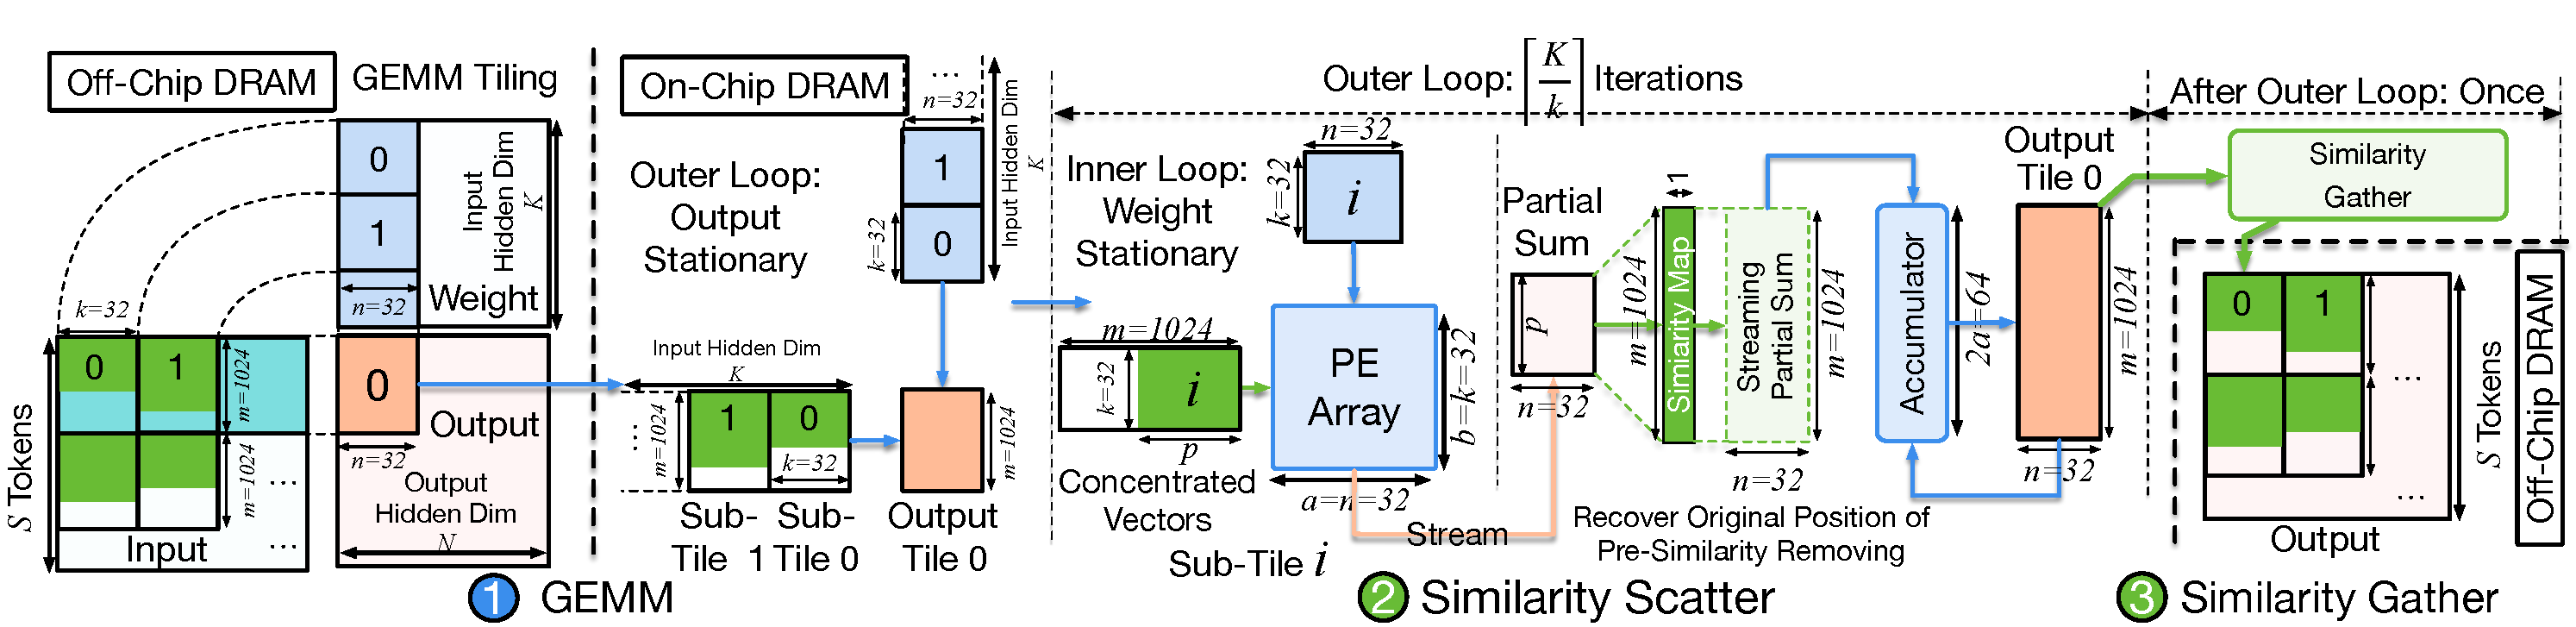
\includegraphics[width=0.98\linewidth]{figure/sic_scatter.pdf}
    % \vspace{-3mm}
    \caption{GEMM tiling and Similarity Scatter design. (1) GEMM computes over concentrated vectors. (2) Similarity Scatter reconstructs and accumulates vector results using similarity maps. (3) Final output is passed to Similarity Gather once after all iterations in a tile.}
    \label{fig:sic_scatter}
    % \vspace{-5mm}
\end{figure*}



To eliminate these conflicts, we propose a \textbf{conflict-free convolution-style layout}, shown in \Fig{fig:sic_layouter}(2), which deterministically maps each token to a unique bank and offset based on its FHW position. 
Given frame index $f$, row $r$, and column $c$, the memory bank and address are computed as:
\vspace{-1mm}
\[
\texttt{Bank} = f \bmod 2 \times 4 + r \bmod 2 \times 2 + c \bmod 2,
\]
\vspace{-3mm}
\[
\texttt{Offset} = \left\lfloor \frac{r}{2} \right\rfloor \times \left\lceil \frac{W}{2} \right\rceil + \left\lfloor \frac{c}{2} \right\rfloor,
\]
where $W$ is the width of the frame. 
This mapping guarantees that all 8 vectors in any $2 \times 2 \times 2$ block reside in distinct memory banks and can be read simultaneously without contention.

\textbf{Key Insight:}  
Unlike traditional approaches that duplicate inputs to avoid access conflicts, our layout achieves fully parallel, conflict-free access \textit{without any data replication}. 
This enables streaming similarity matchers to operate in parallel across tiles and spatial regions, scaling throughput without modifying the GEMM pipeline. 
The layouter thus plays a critical role in supporting parallel similarity execution and maintaining high utilization.

\subsection{Similarity Scatter}
\label{subsec:scatter}

\textbf{GEMM Tiling for Concentrated Vectors.}
As shown in \Fig{fig:sic_scatter}(1), Similarity Scatter operates on the concentrated vectors generated from earlier stages. 
Since only a subset of the original $m=1024$ tokens is retained in each tile ($p < 1024$), the input to this GEMM stage is \textbf{logically sparse} but \textbf{structurally dense}. 
To maintain compatibility with standard systolic-array architectures, GEMM is performed using a conventional tiling scheme with dimensions $m=1024$ and $n=32$.
The GEMM execution follows a two-level nested loop structure:
The \textbf{outer loop} adopts an \textit{output-stationary} dataflow, keeping the $m \times n$ output tile resident on-chip to accumulate results across the $K$ dimension.
The \textbf{inner loop} follows a \textit{weight-stationary} strategy, loading one $k \times n$ weight sub-tile into the PE array while streaming in a $p \times k$ sub-tile of concentrated input vectors.

Each inner loop iteration computes partial products and generates one $a$-dimensional partial sum vector per cycle. Our vector size 32 matches with the $k$ tile size and array height $b$, ensuring full utilization of the PE array.
These vectors are streamed out and accumulated over successive iterations to form the final tile result.
The key advantage arises from the reduced number of active input vectors ($p < 1024$), which significantly lowers the computational workload. 
However, since different sub-tiles may have different subsets of concentrated vectors, each possibly representing multiple original tokens, direct accumulation would produce incorrect outputs due to semantic aliasing.

\textbf{Similarity Scatter and Gather.}
To resolve this, we introduce the \textbf{Similarity Scatter} module, illustrated in \Fig{fig:sic_scatter}(2). 
After each GEMM step, the generated partial sums are streamed into a temporary buffer. 
Using the similarity map from previous layer's the gather phase (see \Sec{subsec:gather}), each partial sum is replicated and redistributed to its associated original token indices, reconstructing the full $m=1024$ output.
This scattered output is then accumulated into an output-stationary buffer spanning all outer loop iterations. 
To maintain throughput parity, we employ a $2a$-wide accumulator (e.g., 64 when $a = 32$), enabling concurrent accumulation of reconstructed vectors and streaming outputs. 
The reconstruction process is performed in-place, incurs negligible overhead, and does not require additional memory allocation.

Upon completing all $\left\lceil \frac{K}{k} \right\rceil$ outer loop iterations, the fully accumulated output tile is passed to the \textbf{Similarity Gather} unit (see \Sec{subsec:gather}), shown in \Fig{fig:sic_scatter}(3). 
This final stage is invoked only once per tile after GEMM concludes and lies entirely off the critical compute path.

In summary, by executing GEMM on a compact set of concentrated vectors, \proj{} achieves substantial compute savings.  
Through the Similarity Scatter module, it efficiently reconstructs full output tiles with minimal accuracy loss, and the final gather stage removes vector-level redundancy.  
This hardware-oriented, vector-granular compression strategy ensures high compute efficiency while preserving model fidelity.  
Our evaluation shows that the additional logic is lightweight and does not impact GEMM throughput, making it a key enabler of \proj{}'s performance advantage.
